\newpage
\subsubsection{Stockage des questions dans différents dossiers}
Nous avons choisi pour plusieurs raisons(clarté,modulabilité,etc...)d'organiser l'ensemble des fichiers sources du jeu en dossiers et sous-dossiers de la manière suivante:\begin{itemize}
			\item Un dossier par Univers, ici "Univers1" mais nous aurions tout aussi bien en créer plusieurs.
			\item Un dossier par Mondes qui sont contenues dans le fichier de L'Univers. Ici les mondes sont "IleDepart","NorthIsland","WestIsland","SouthIsland" et "EastIsland".
			\item Un dossier par Zones qui sont relatifs au monde au quel elles appartiennent. Le nom de ces dossiers est par exemple "plage","cabane",etc...
			\item Un fichier par question dans chaque dossier de zones.La question dans une zone sera choisie aléatoirement parmi les fichiers présents dans le dossier.   
	     \end{itemize}
\begin{figure}[h]
 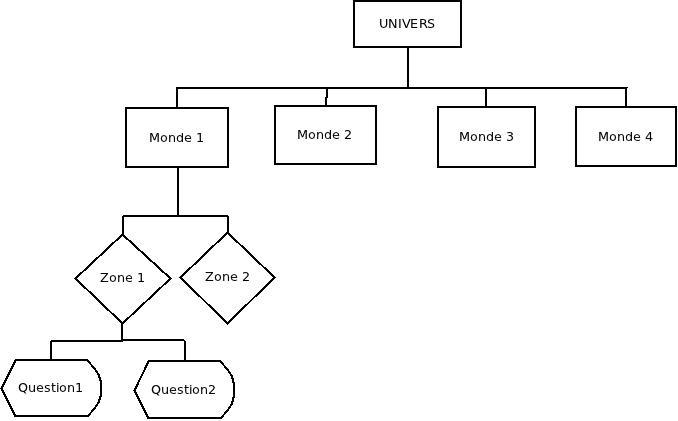
\includegraphics[scale=0.8]{./figures/hier.jpeg}
	\caption{Schéma de l'organisation en dossier }
\end{figure}